
\section{Parallel and Distributed Database Design}

\subsection{Justification for a Distributed and Parallel Design}

The system requires an infrastructure capable of operating \textbf{efficiently, continuously, and at scale} in the face of the following challenges:

\begin{itemize}[leftmargin=1.5em]
  \item \textbf{High-frequency data ingestion:} Every 10 minutes, data is received from multiple external air quality sources.
  \item \textbf{Complex analytical queries:} The system must process historical trends, pollutant groupings, locations, and time ranges.
  \item \textbf{Concurrent access from multiple regions:} Users such as citizens, government agencies, and researchers interact from different geographic zones.
  \item \textbf{Storage of large historical volumes:} The system is expected to store years of station data, resulting in high volumes of temporal and geospatial information.
  \item \textbf{Continuous availability:} The system must run uninterrupted, with fault tolerance and operational continuity for both reads and writes.
\end{itemize}

To address these challenges, a \textbf{distributed and parallel architecture} is proposed, which includes:

\begin{itemize}[leftmargin=1.5em]
  \item \textbf{Horizontal scalability:} The ability to add nodes or instances as data volume or user demand grows.
  \item \textbf{High availability:} Through replication, redundancy, and load balancing.
  \item \textbf{Load separation:} Decoupling ingestion, querying, and data visualization processes to prevent bottlenecks or blocking operations.
\end{itemize}

\subsection{High-Level Design}

\subsubsection{Data Distribution and Segmentation}

\begin{itemize}[leftmargin=1.5em]
  \item \textbf{Temporal partitioning:} Data is divided based on collection time (e.g., by week or month), facilitating historical queries and storage management.
  \item \textbf{Geographic segmentation:} Data is distributed by region or country, enabling localized queries, improved performance, and compliance with regional regulations.
  \item \textbf{User- or entity-based fragmentation:} Configurations, alerts, and preferences are distributed based on user or institution identifiers, ensuring balanced load and fast access.
\end{itemize}

\subsubsection{General Diagram of Distributed Architecture}

\begin{figure}[H]
  \centering
  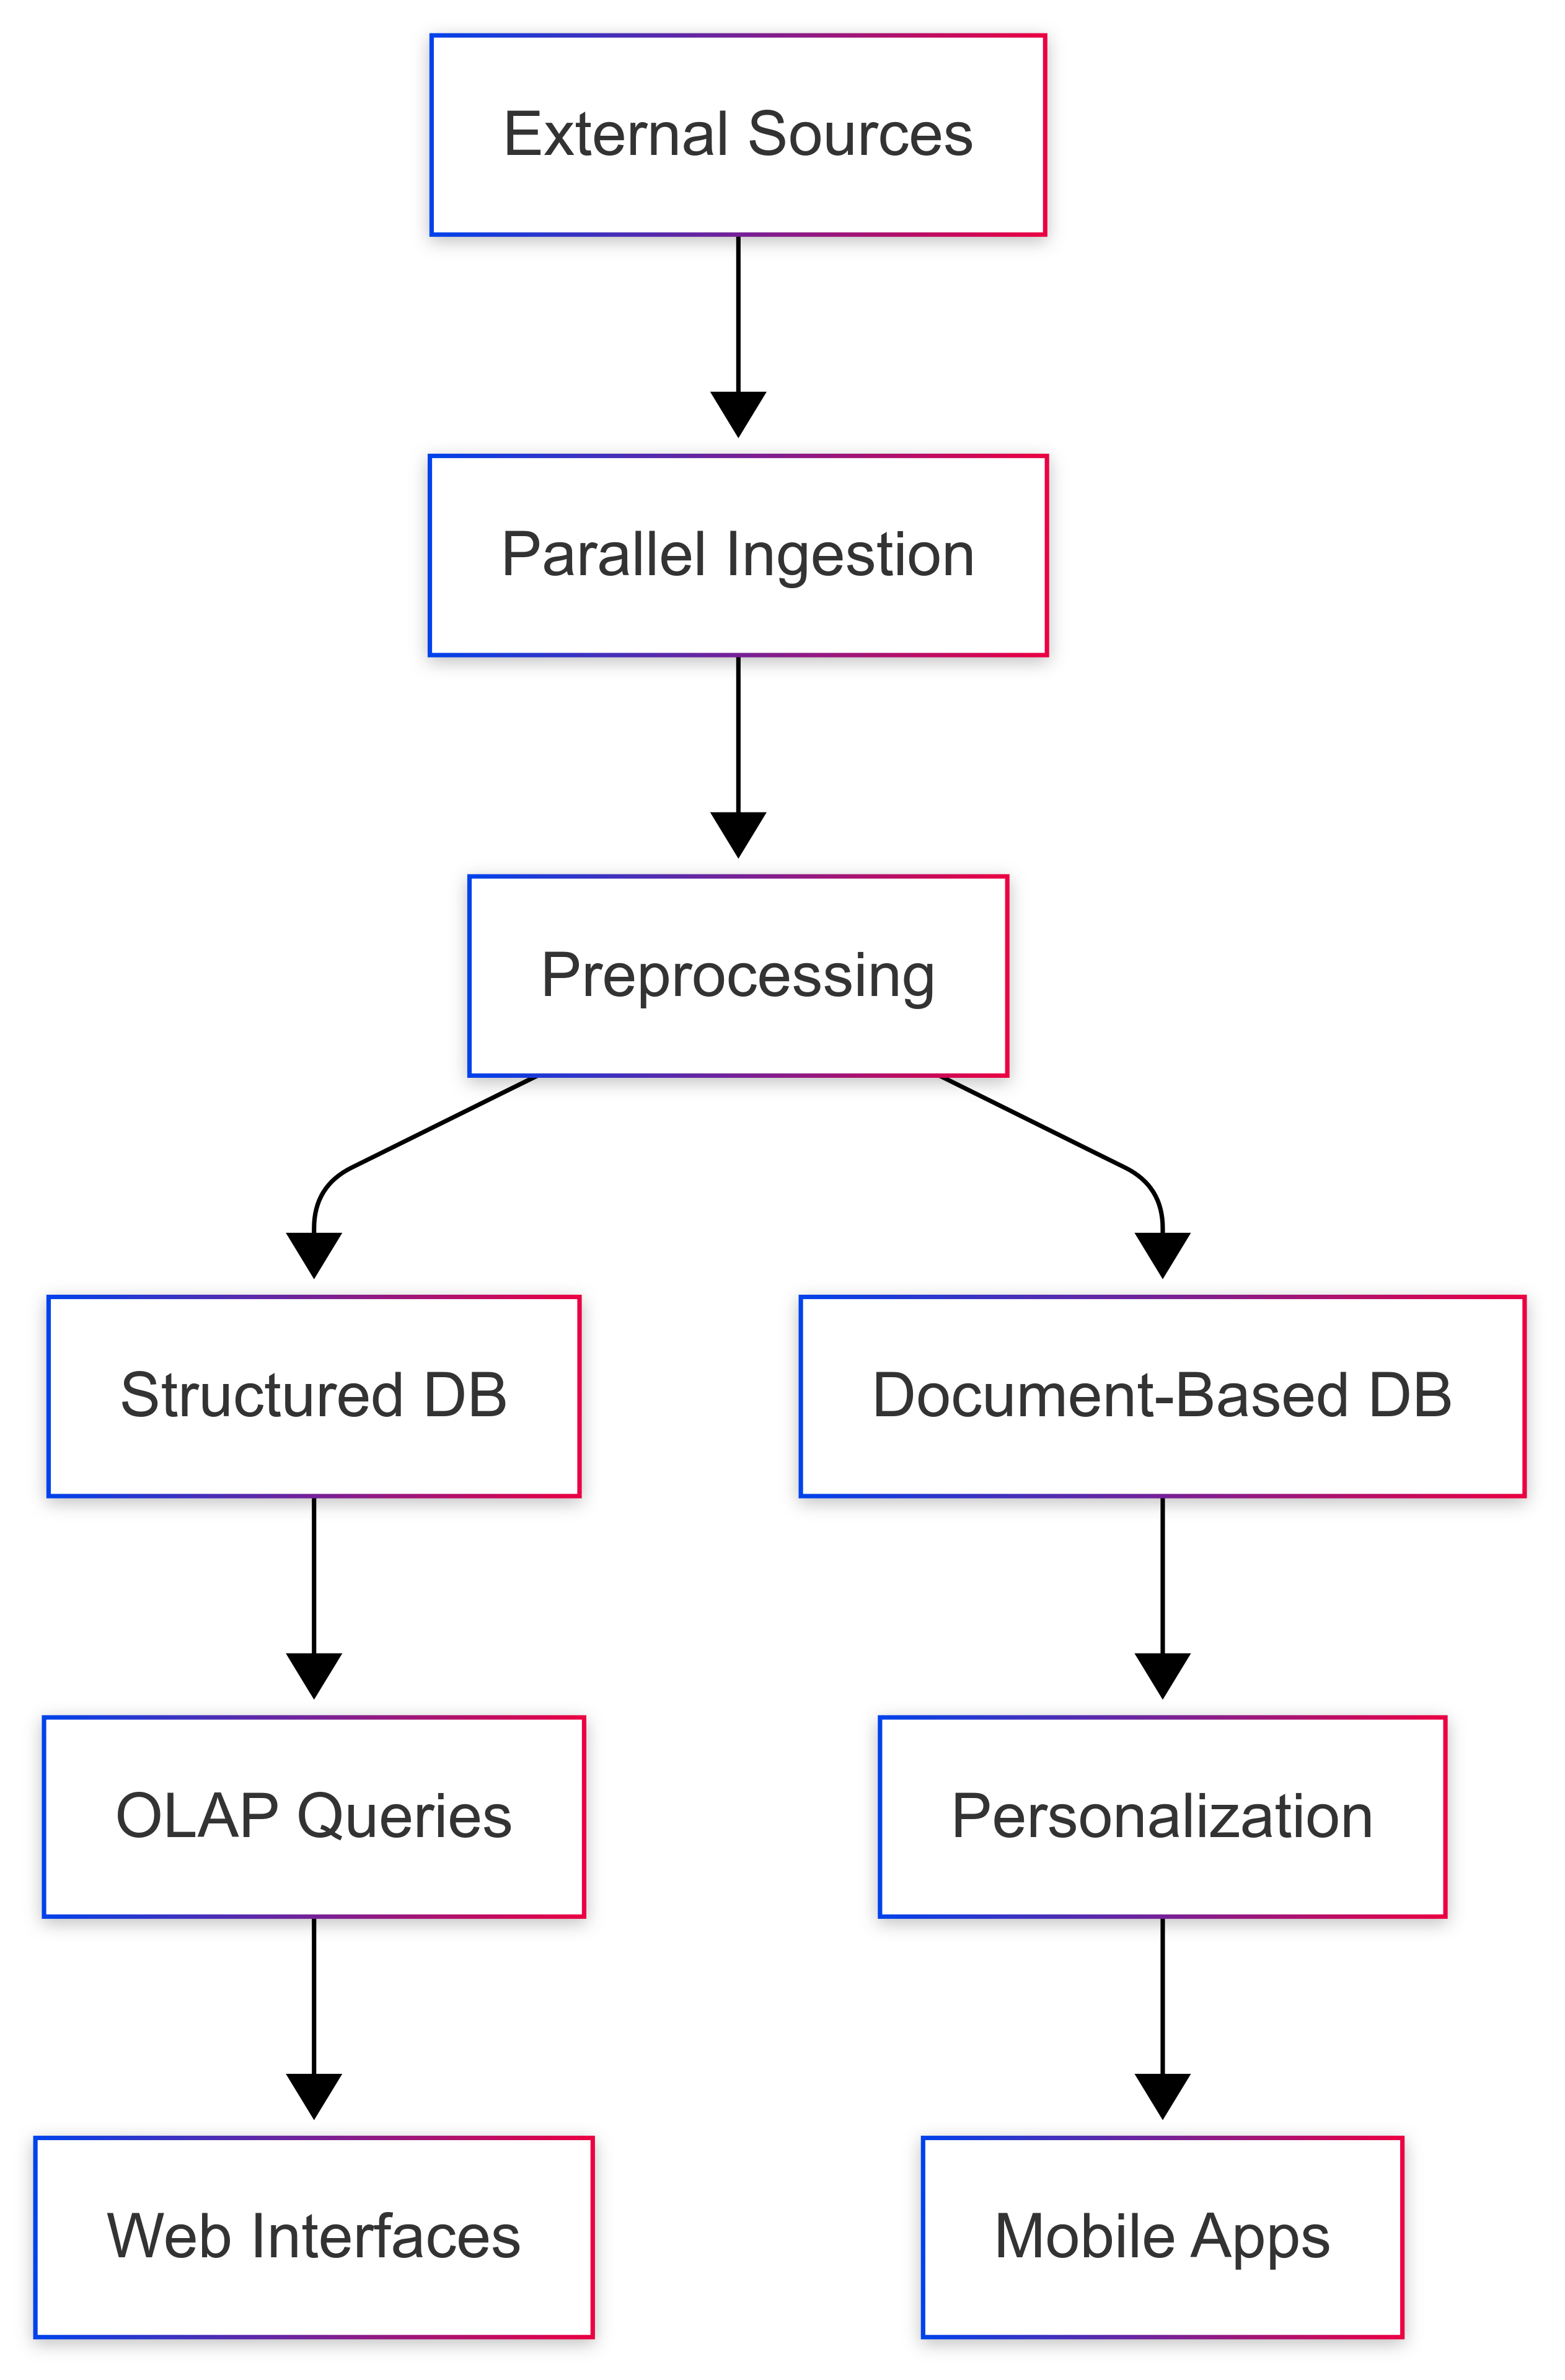
\includegraphics[width=0.8\textwidth]{Imagenes/distributed.png}
  \caption{High-level Distributed Database Architecture}
\end{figure}


\subsection{Parallelism Strategies}

\begin{longtable}{@{}p{4cm}p{6cm}p{6cm}@{}}
\toprule
\textbf{Area} & \textbf{Applied Technique} & \textbf{Expected Benefit} \\
\midrule
Query processing & Parallel execution of aggregations, filters, and groupings & Reduces response time for complex reports \\
Data ingestion & Independent processes per data source & Allows simultaneous ingestion without degrading overall performance \\
Real-time visualization & Non-blocking updates of precomputed views & Ensures smooth access without intermediate calculation delays \\
Distributed storage & Load distribution across multiple nodes or regions & Improves performance and availability in case of failures \\
Concurrent querying & Dedicated read replicas for reporting or BI & Separates analytical load from daily transactional processing \\
Highly dynamic data & Segmentation based on user or device & Reduces latency for personalized operations \\
\bottomrule
\end{longtable}

\subsection{Technical Justification Based on Requirements}

\begin{longtable}{@{}p{6.5cm}p{8.5cm}@{}}
\toprule
\textbf{System Requirement} & \textbf{Adopted Architectural Approach} \\
\midrule
Continuous data ingestion & Parallel processing per input source \\
24/7 high availability & Replication and load balancing across distributed nodes \\
Real-time access (<2 seconds) & Optimized queries over precomputed views \\
Massive personalization & Horizontal segmentation of user data \\
Historical reports with millions of records & Time-based partitioning + distributed execution \\
Geographic and demographic expansion & Regional sharding and request load balancing by zone \\
Read/write separation & Role-based division between query and processing databases \\
\bottomrule
\end{longtable}